\chapter{Git Hook Bash Script}
\begin{figure}[htp]
    \centering
    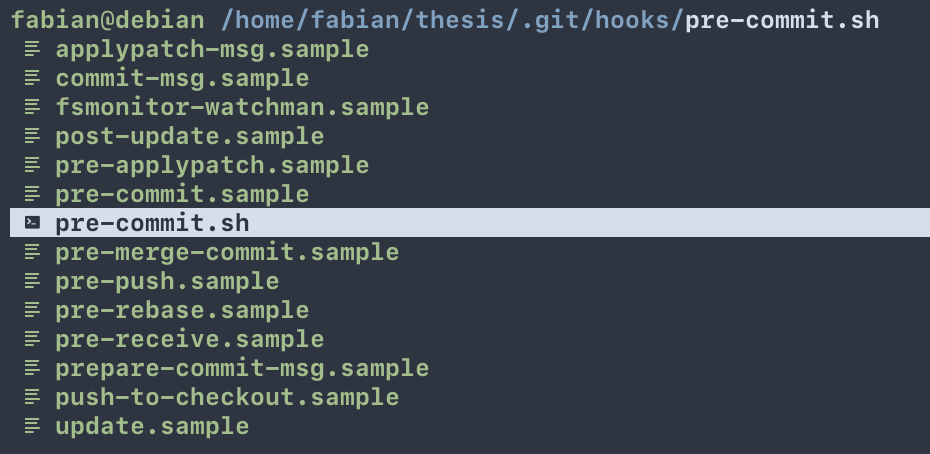
\includegraphics[width=1\columnwidth]{./latex/appendix/placeholder}
    \caption{Bash script (executed before to Git Commit)}
    \label{fig:bash}
\end{figure}

\newpage


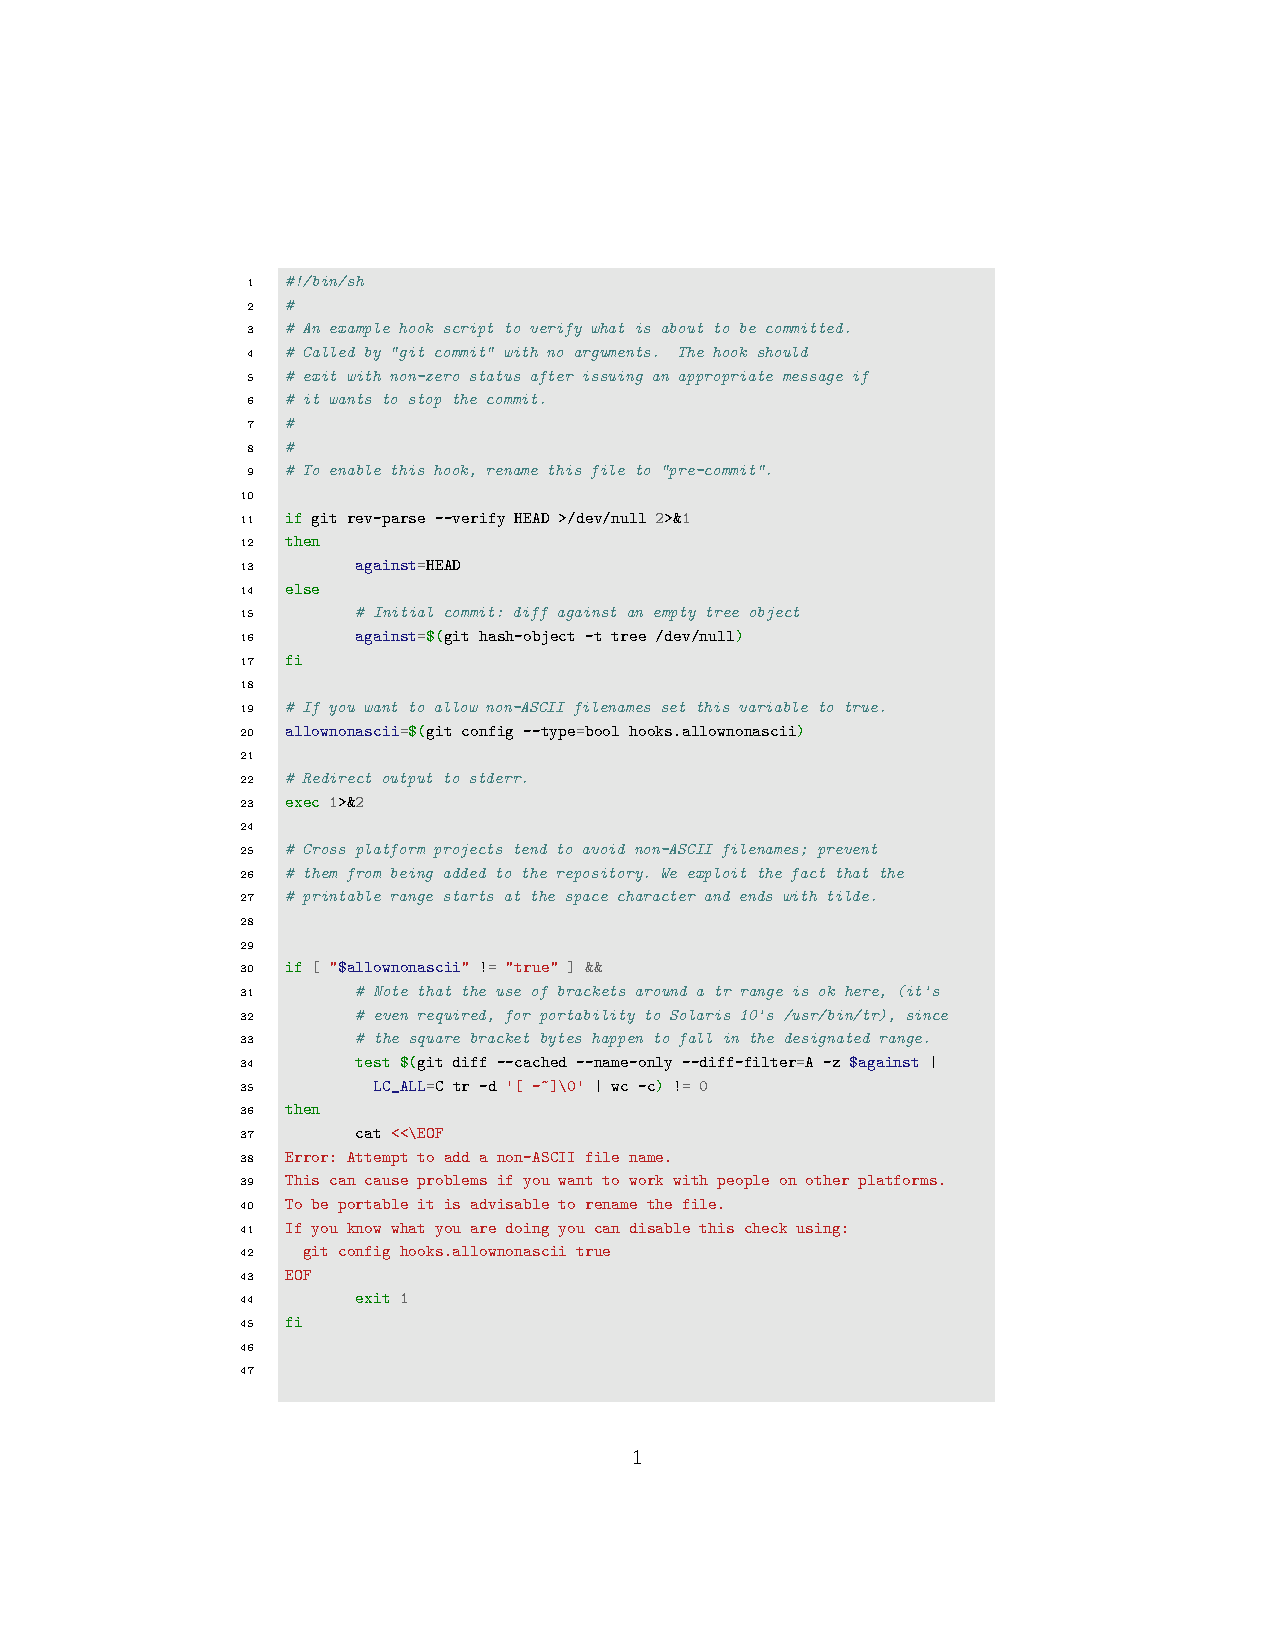
\includepdf[page=-]{latex/appendix/hook}
\chapter{Formalization of Gherkin Specifications}
\newpage

\begin{figure}[htp]
    \centering
    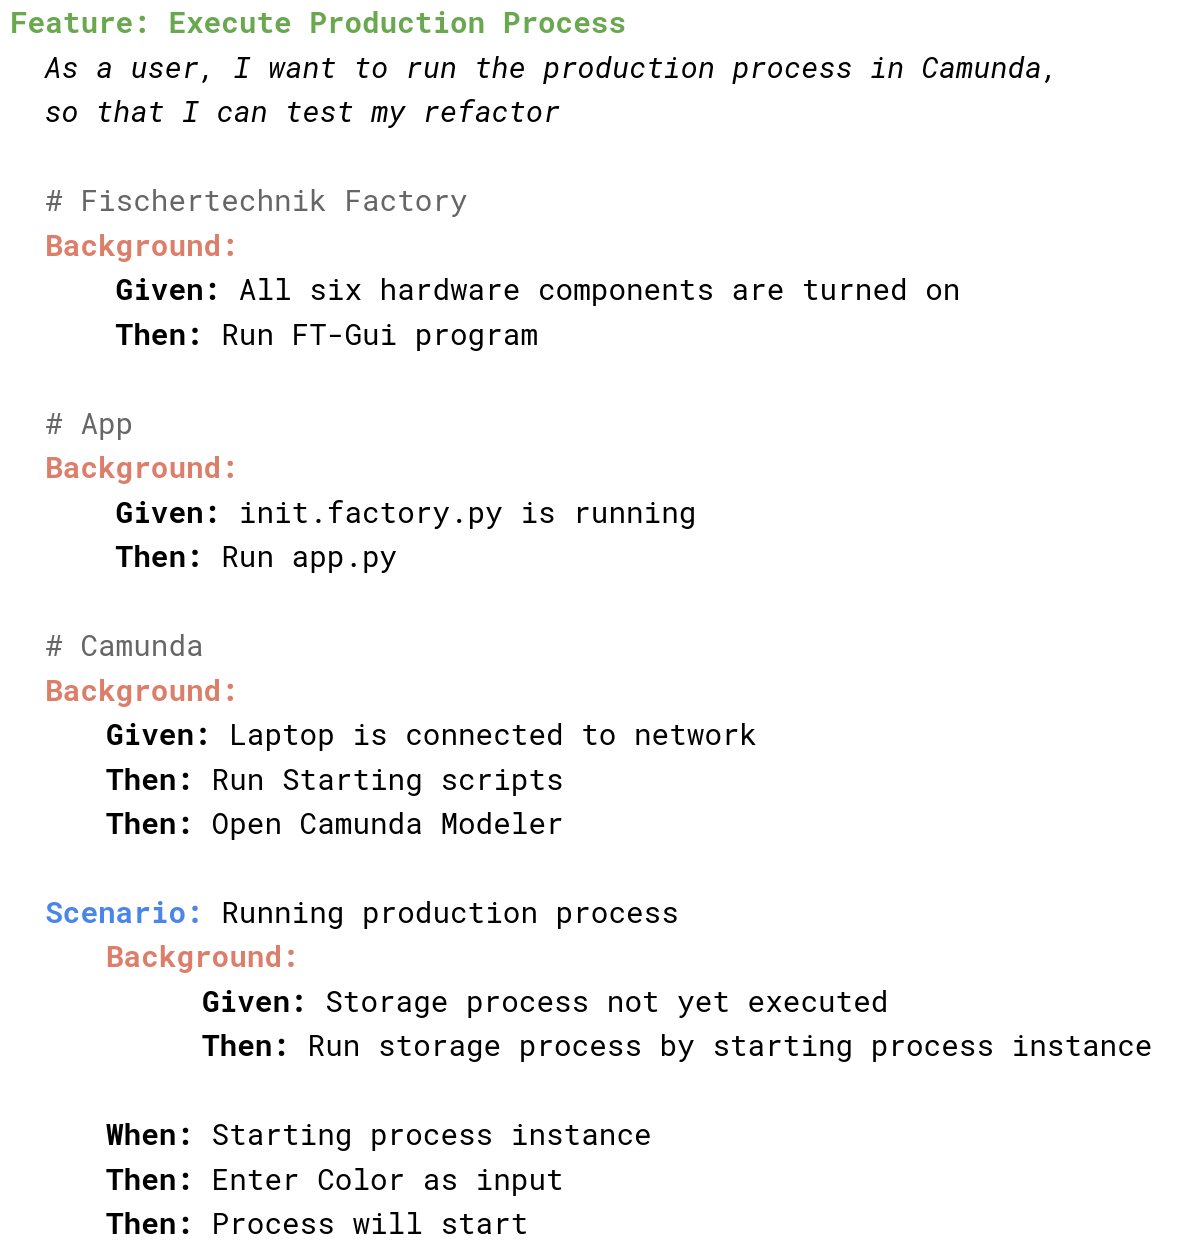
\includegraphics[width=0.7\columnwidth]{./latex/appendix/gherkin}
    \caption{Gherkin Specifications applied to software system}
    \label{appendix:gherkin}
\end{figure}

As seen in the specifications above, one can observe multiple prerequisites that are necessary due to having hardware. This amount of detail is critical when wanting to reproduce this process at a later time. Even though, some specifications might seem self-evident, only then we can diminish the ambiguity associated with testing CPS. Each step must start with one of the Gherkin predefined keywords \emph{Given, When, Then, And, or But} providing the necessary structure. Such structure enables to formulate requirements that can translate to preconditions, user actions, and outcomes of the procedure.

\chapter{Sonargraph Graphical Interface}
\newpage

\section{Metric View}
\begin{figure}[htp]
    \centering
    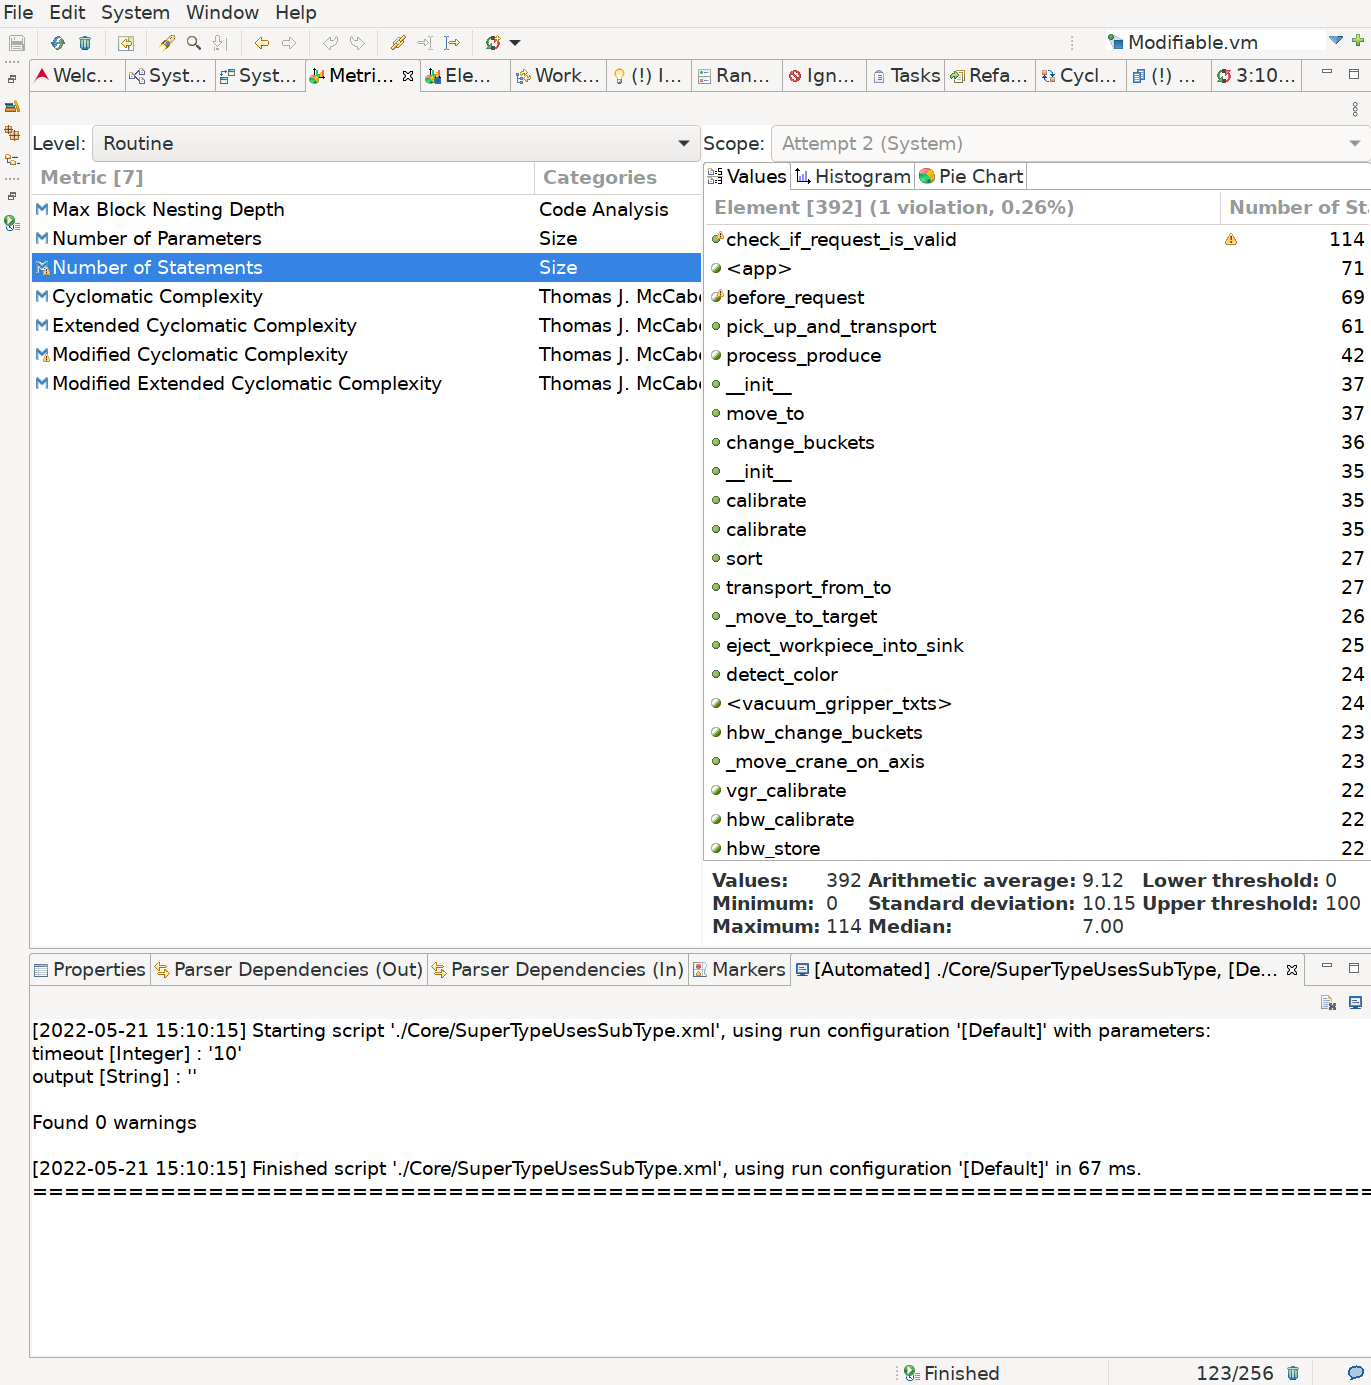
\includegraphics[width=\textwidth, frame]{./latex/appendix/sonar-metrics}
    \caption{Evaluation of Metrics in Sonargraph}
    \label{appendix:metrics}
\end{figure}

\newpage
\section{Duplications View}
\begin{figure}[htp]
    \centering
    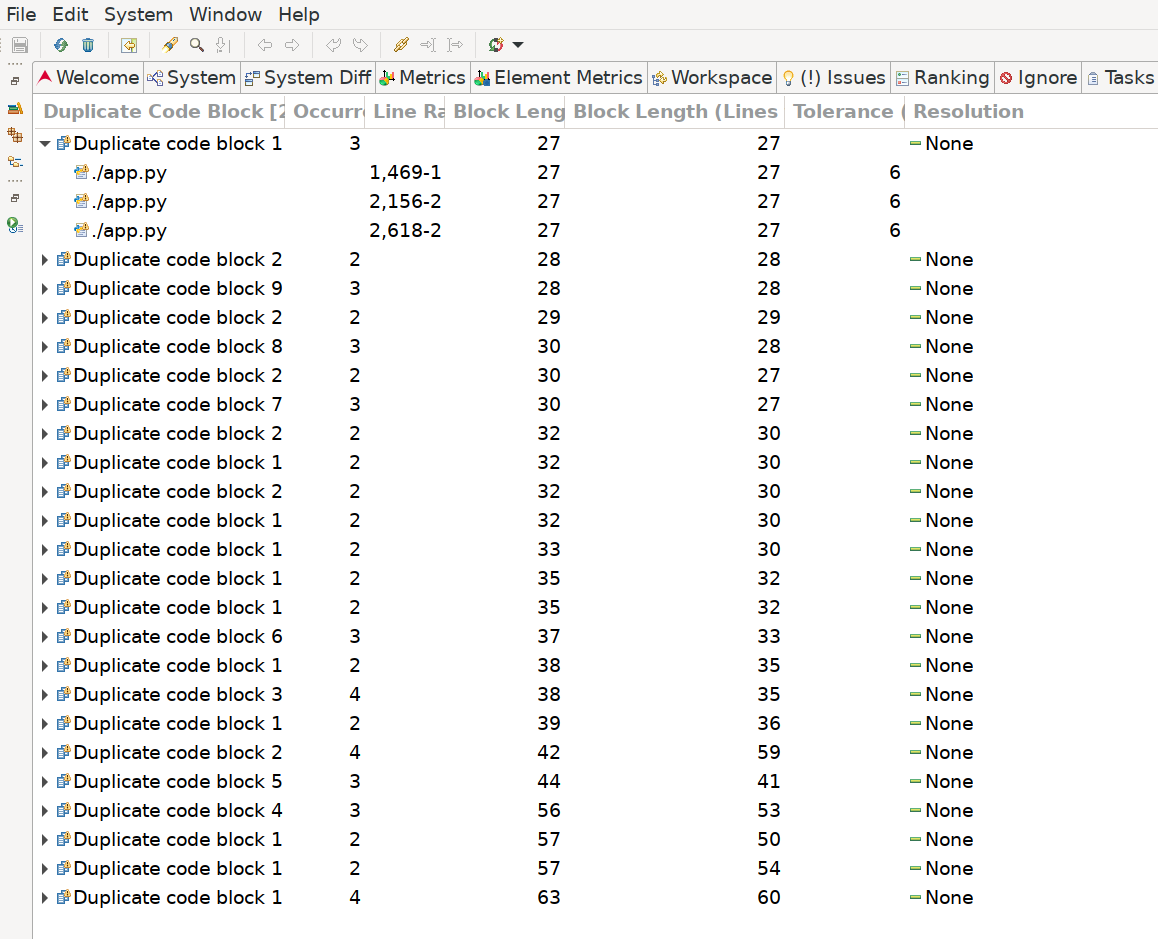
\includegraphics[width=\textwidth, frame]{./latex/appendix/duplications}
    \caption{Overview of Code Duplications}
    \label{appendix:duplications}
\end{figure}

\newpage
\section{Side by Side comparison of duplicates}
\begin{figure}[htp]
    \centering
    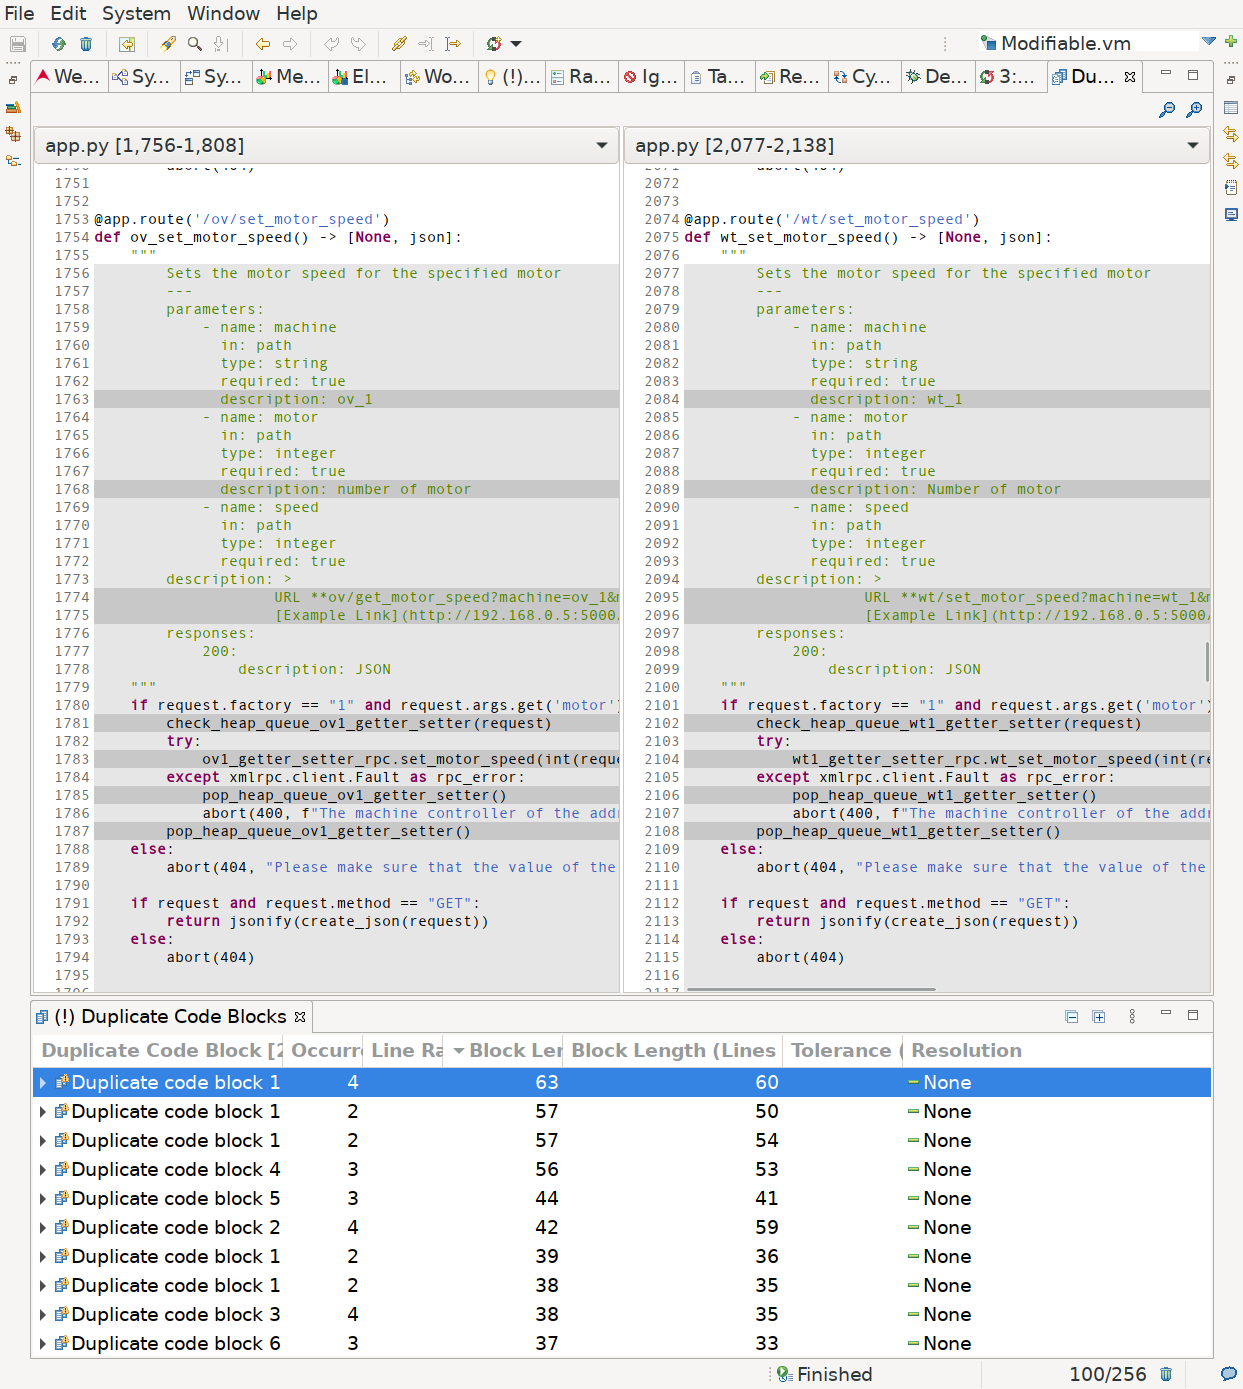
\includegraphics[width=0.9\columnwidth, frame]{./latex/appendix/duplicate-view}
    \caption{Duplicated Code Block Source View}
    \label{appendix:duplications-view}
\end{figure}